\documentclass{article}\usepackage[]{graphicx}\usepackage[]{color}
%% maxwidth is the original width if it is less than linewidth
%% otherwise use linewidth (to make sure the graphics do not exceed the margin)
\makeatletter
\def\maxwidth{ %
  \ifdim\Gin@nat@width>\linewidth
    \linewidth
  \else
    \Gin@nat@width
  \fi
}
\makeatother

\definecolor{fgcolor}{rgb}{0.345, 0.345, 0.345}
\newcommand{\hlnum}[1]{\textcolor[rgb]{0.686,0.059,0.569}{#1}}%
\newcommand{\hlstr}[1]{\textcolor[rgb]{0.192,0.494,0.8}{#1}}%
\newcommand{\hlcom}[1]{\textcolor[rgb]{0.678,0.584,0.686}{\textit{#1}}}%
\newcommand{\hlopt}[1]{\textcolor[rgb]{0,0,0}{#1}}%
\newcommand{\hlstd}[1]{\textcolor[rgb]{0.345,0.345,0.345}{#1}}%
\newcommand{\hlkwa}[1]{\textcolor[rgb]{0.161,0.373,0.58}{\textbf{#1}}}%
\newcommand{\hlkwb}[1]{\textcolor[rgb]{0.69,0.353,0.396}{#1}}%
\newcommand{\hlkwc}[1]{\textcolor[rgb]{0.333,0.667,0.333}{#1}}%
\newcommand{\hlkwd}[1]{\textcolor[rgb]{0.737,0.353,0.396}{\textbf{#1}}}%

\usepackage{framed}
\makeatletter
\newenvironment{kframe}{%
 \def\at@end@of@kframe{}%
 \ifinner\ifhmode%
  \def\at@end@of@kframe{\end{minipage}}%
  \begin{minipage}{\columnwidth}%
 \fi\fi%
 \def\FrameCommand##1{\hskip\@totalleftmargin \hskip-\fboxsep
 \colorbox{shadecolor}{##1}\hskip-\fboxsep
     % There is no \\@totalrightmargin, so:
     \hskip-\linewidth \hskip-\@totalleftmargin \hskip\columnwidth}%
 \MakeFramed {\advance\hsize-\width
   \@totalleftmargin\z@ \linewidth\hsize
   \@setminipage}}%
 {\par\unskip\endMakeFramed%
 \at@end@of@kframe}
\makeatother

\definecolor{shadecolor}{rgb}{.97, .97, .97}
\definecolor{messagecolor}{rgb}{0, 0, 0}
\definecolor{warningcolor}{rgb}{1, 0, 1}
\definecolor{errorcolor}{rgb}{1, 0, 0}
\newenvironment{knitrout}{}{} % an empty environment to be redefined in TeX

\usepackage{alltt}

\input{c:/aaaWork/zGnrlLatex/GnrlPreamble}
\hypersetup{pdftitle = RFish Midwest 2012 Notes}
\input{c:/aaaWork/zGnrlLatex/JustRPreamble}
\IfFileExists{upquote.sty}{\usepackage{upquote}}{}
\begin{document}
  \title{Tobin Harbor Brook Trout Report}
  \author{\vspace{-12pt}Derek H. Ogle}
  \date{\vspace{-12pt}\today}
  \maketitle



\section*{Introduction}
Brook trout are important.  Isle Royale is a fun place to sample fish.

\section*{Methods}
We electrofished.  Caught and aged fish.  Used a catch curve analysis to estimate the instantaneous mortality rate.

\section*{Results}


A total of 604 brook trout were captured.  The maximum catch of 182 occurred at age-1.  The instantaneous mortality computed for ages 1 to 5 was 0.253 with a 95\% confidence interval from 0.205 to 0.302 \figrefp{fig:CatchCurve}.

\begin{knitrout}
\definecolor{shadecolor}{rgb}{0.969, 0.969, 0.969}\color{fgcolor}\begin{figure}[h]

{\centering 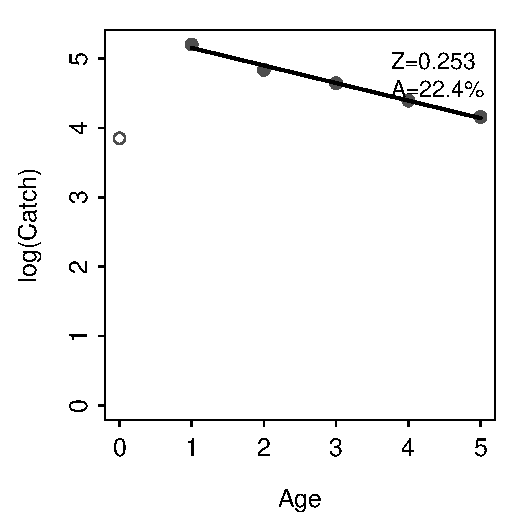
\includegraphics[width=.4\linewidth]{Figs/CatchCurve-1} 

}

\caption[Log catch versus age for Tobin Harbor Brook Trout, with the ages used for estimating Z shown]{Log catch versus age for Tobin Harbor Brook Trout, with the ages used for estimating Z shown.}\label{fig:CatchCurve}
\end{figure}


\end{knitrout}

\section*{Discussion}
We did great work.

\end{document}
